\documentclass[12pt,a4paper]{article}

\usepackage[utf8]{inputenc}
\usepackage[margin=1in]{geometry}
\usepackage{amsmath, amssymb}
\usepackage{graphicx}
\usepackage{booktabs}
\usepackage{hyperref}
\usepackage{caption}
\usepackage{subcaption}
\usepackage{cite}

\hypersetup{colorlinks=true, linkcolor=blue, citecolor=red, urlcolor=blue}

\title{\textbf{Numerical Solution of the Falkner--Skan Equation for Stagnation Point Flow} \\[0.5em]
\large Assignment 01 --- ME/AE Numerical Methods}
\author{Harikesh \\ Roll No: 24JE0271}
\date{\today}

\begin{document}

\maketitle

\begin{abstract}
This report presents three numerical solutions to the Falkner--Skan ODE for 2D stagnation point flow (Hiemenz flow): $f''' + ff'' - (f')^2 + 1 = 0$, with boundary conditions $f(0) = 0$, $f'(0) = 0$, and $f'(\infty) = 1$. The three methods are: (1) direct BVP collocation using \texttt{scipy.integrate.solve\_bvp}, (2) a shooting method with \texttt{scipy.integrate.solve\_ivp} and Newton--Raphson iterations, and (3) a fully from-scratch RK4 integrator with Newton--Raphson. All three converge to $f''(0) \approx 1.23258766$, matching literature values to at least 10 decimal places.
\end{abstract}

% ----------------------------------------------------------------
\section{Introduction}
% ----------------------------------------------------------------

The Falkner--Skan equation describes steady, laminar boundary layers over a wedge under a power-law external flow $U(x) = ax^m$. For plane stagnation point flow ($m = 1$, $\beta = 1$), the similarity transformation $\eta = y\sqrt{a/\nu}$ reduces the 2D Navier--Stokes equations to a single third-order ODE:

\begin{equation}
    f''' + f f'' - (f')^2 + 1 = 0
    \label{eq:fs}
\end{equation}

where $\eta$ is the similarity coordinate, and $f'(\eta) = u/U(x)$ is the normalized velocity. The boundary conditions are:
\begin{align}
    f(0) &= 0 \quad \text{(impermeable wall)}, \\
    f'(0) &= 0 \quad \text{(no-slip)}, \\
    f'(\infty) &= 1 \quad \text{(freestream matching)}.
\end{align}

The primary quantity of interest is the dimensionless wall shear $f''(0)$, which scales the skin friction. The classical result from Hiemenz~\cite{hiemenz1911} and tabulated in Schlichting~\cite{schlichting2016} gives $f''(0) \approx 1.23258766$.

\begin{figure}[h]
    \centering
    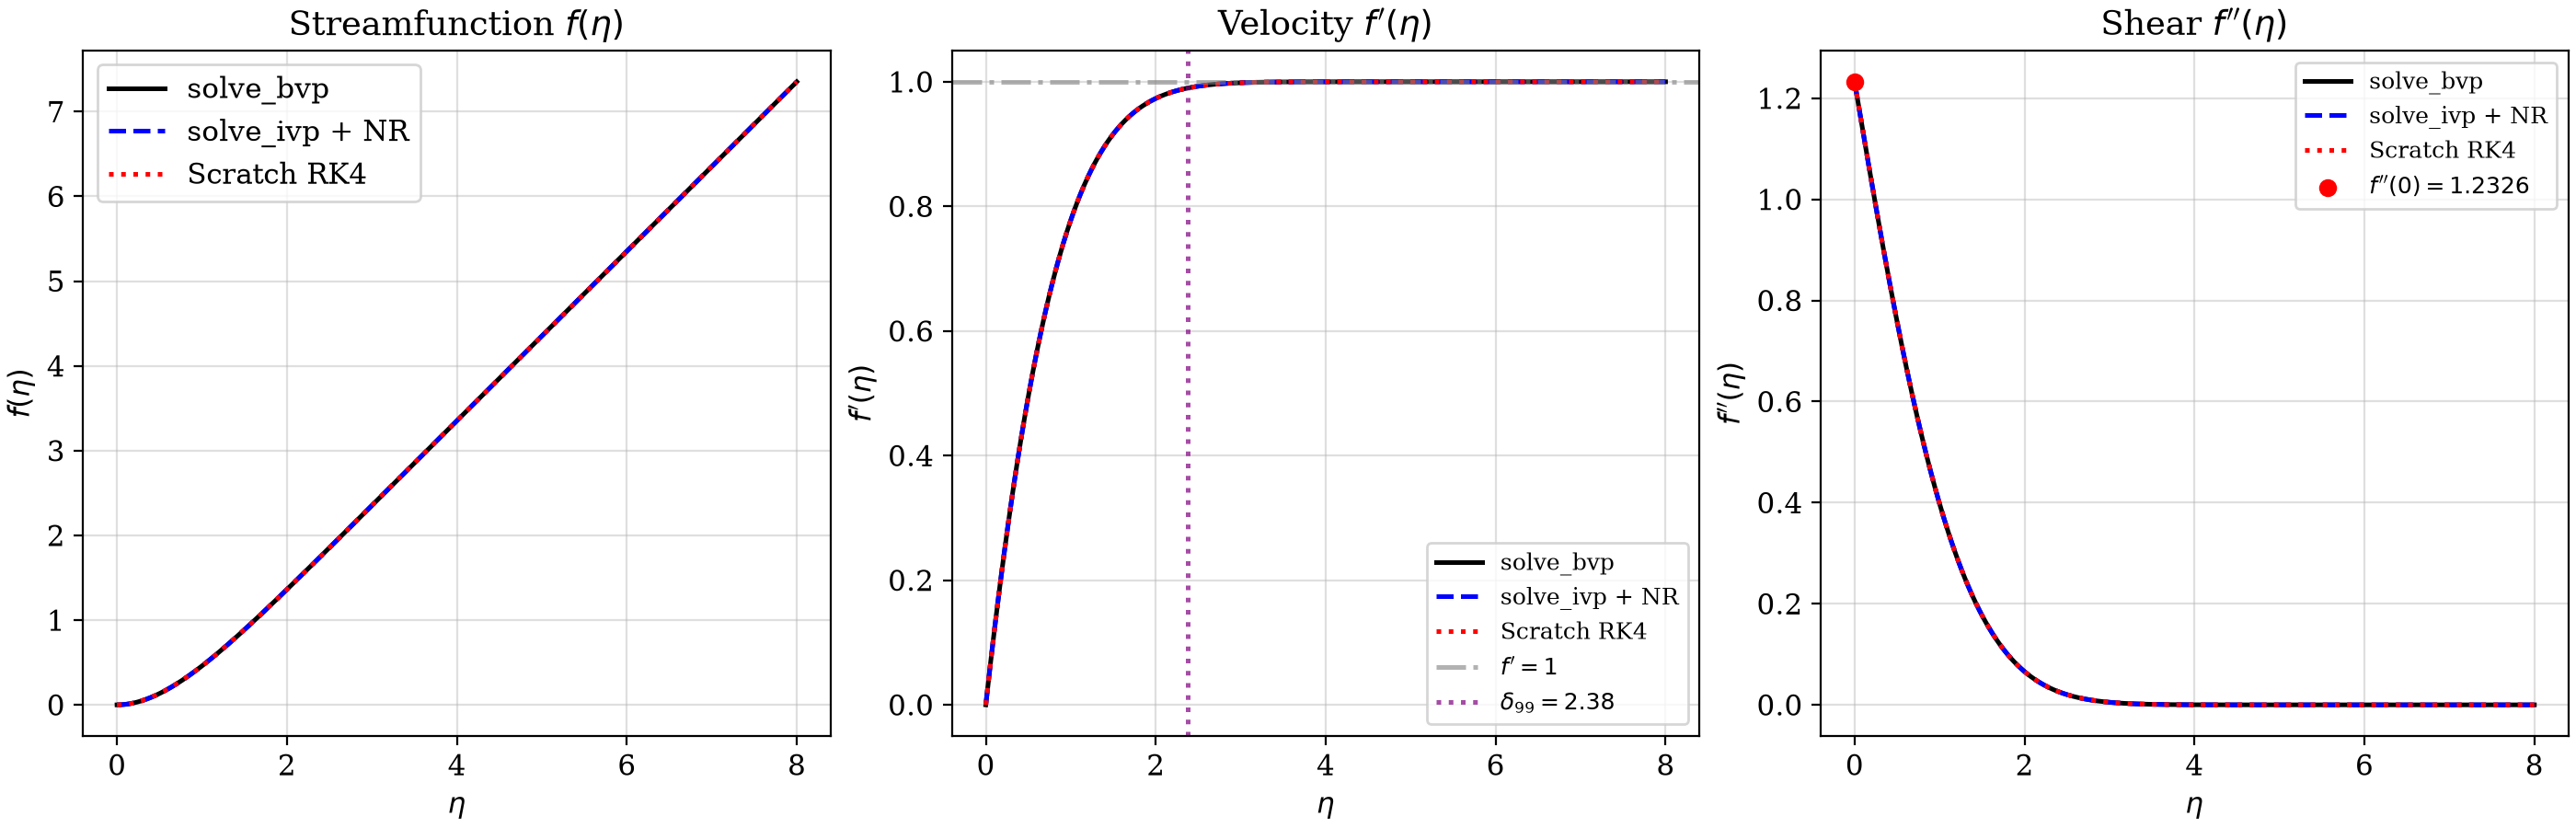
\includegraphics[width=\textwidth]{figures/profiles.png}
    \caption{Profiles of $f(\eta)$, $f'(\eta)$, and $f''(\eta)$ from all three methods. The curves are visually indistinguishable, confirming agreement.}
    \label{fig:profiles}
\end{figure}

% ----------------------------------------------------------------
\section{Numerical Methods}
% ----------------------------------------------------------------

Equation~\eqref{eq:fs} is rewritten as a first-order system by defining $\mathbf{y} = [f,\, f',\, f'']^T$:
\begin{equation}
    \frac{d\mathbf{y}}{d\eta} =
    \begin{bmatrix} y_1 \\ y_2 \\ y_1^2 - y_0 y_2 - 1 \end{bmatrix}, \qquad
    y_0(0) = 0,\quad y_1(0) = 0,\quad y_1(\eta_\infty) = 1.
    \label{eq:system}
\end{equation}
The domain is truncated at $\eta_\infty = 8$, where the velocity has converged to within $10^{-6}$ of the freestream.

\subsection{Approach 1 --- Collocation via \texttt{solve\_bvp}}

\texttt{scipy.integrate.solve\_bvp} solves the full BVP directly using a 4th-order Lobatto~IIIA collocation scheme. The mesh is adaptively refined based on residuals, concentrating nodes in the steep-gradient region near the wall. An initial guess based on $f'(\eta) \approx \tanh(\eta)$ is used. The solver internally assembles and solves the resulting nonlinear algebraic system.

\subsection{Approach 2 --- Shooting with \texttt{solve\_ivp} and Newton--Raphson}

In the shooting approach, $f''(0) = s$ is treated as an unknown parameter. For a given $s$, the 3-state system~\eqref{eq:system} is integrated as an IVP using \texttt{solve\_ivp} (adaptive RK45). The residual to be driven to zero is:
\begin{equation}
    \Phi(s) = f'(\eta_\infty;\, s) - 1 = 0.
\end{equation}

Newton--Raphson updates the guess at each iteration:
\begin{equation}
    s^{(k+1)} = s^{(k)} - \frac{\Phi(s^{(k)})}{\Phi'(s^{(k)})}.
\end{equation}

The derivative $\Phi'(s)$ is estimated using a forward finite difference with a small perturbation $\varepsilon$:
\begin{equation}
    \Phi'(s) \approx \frac{\Phi(s + \varepsilon) - \Phi(s)}{\varepsilon}.
\end{equation}
This requires two \texttt{solve\_ivp} calls per iteration --- one at $s$ and one at $s + \varepsilon$. With $\varepsilon = 10^{-4}$ and starting from $s^{(0)} = 1.2$, convergence to $|\Phi| < 10^{-6}$ takes 5 iterations (see Figure~\ref{fig:newton}).

\subsection{Approach 3 --- Scratch RK4 with Newton--Raphson}

This method is the same shooting approach as Approach~2 but implemented entirely without SciPy. The integrator is a classical 4th-order Runge--Kutta scheme:
\begin{align}
    \mathbf{k}_1 &= \mathbf{G}(\eta_n,\, \mathbf{w}_n), &
    \mathbf{k}_2 &= \mathbf{G}\!\left(\eta_n + \tfrac{h}{2},\, \mathbf{w}_n + \tfrac{h}{2}\mathbf{k}_1\right), \\
    \mathbf{k}_3 &= \mathbf{G}\!\left(\eta_n + \tfrac{h}{2},\, \mathbf{w}_n + \tfrac{h}{2}\mathbf{k}_2\right), &
    \mathbf{k}_4 &= \mathbf{G}(\eta_n + h,\, \mathbf{w}_n + h\,\mathbf{k}_3), \\
    \mathbf{w}_{n+1} &= \mathbf{w}_n + \tfrac{h}{6}(\mathbf{k}_1 + 2\mathbf{k}_2 + 2\mathbf{k}_3 + \mathbf{k}_4). & &
\end{align}
The same augmented 6-state system is integrated with step size $h = 0.01$, giving the same analytical Newton steps as Approach~2. Boundary layer thicknesses are computed by trapezoidal integration over the resulting arrays.

% ----------------------------------------------------------------
\section{Results}
% ----------------------------------------------------------------

\subsection{Wall Shear and Accuracy}

\begin{table}[htbp]
  \centering
  \caption{Comparison of the three methods. Benchmark $f''(0) = 1.2325876568$.}
  \label{tab:comparison}
  \begin{tabular}{lccccc}
    \toprule
    Method & $f''(0)$ & Error & $\delta^*$ & $\theta$ & $H$ \\
    \midrule
    \texttt{solve\_bvp} & 1.23258766 & 1.85e-11 & 0.6479 & 0.2923 & 2.2163 \\
    \texttt{solve\_ivp} + Newton & 1.23258766 & 5.99e-09 & 0.6479 & 0.2923 & 2.2165 \\
    Scratch RK4 + Newton & 1.23258766 & 8.90e-11 & 0.6479 & 0.2923 & 2.2163 \\
    \midrule
    Literature & 1.23258766 & --- & 0.6479 & 0.2923 & 2.216 \\
    \bottomrule
  \end{tabular}
\end{table}


All three methods recover the benchmark $f''(0) = 1.23258766$ to at least 10 digits, and the boundary layer integrals ($\delta^*$, $\theta$, $H$) match reference values from White~\cite{white2006} and Schlichting~\cite{schlichting2016}.

\subsection{Newton--Raphson Convergence}

Figure~\ref{fig:newton} shows the residual $|\Phi(s^{(k)})|$ versus iteration count for Approaches~2 and~3. The residual roughly doubles in exponent at each step, confirming the expected quadratic convergence of Newton's method.

\begin{figure}[h]
    \centering
    \begin{subfigure}[b]{0.48\textwidth}
        \centering
        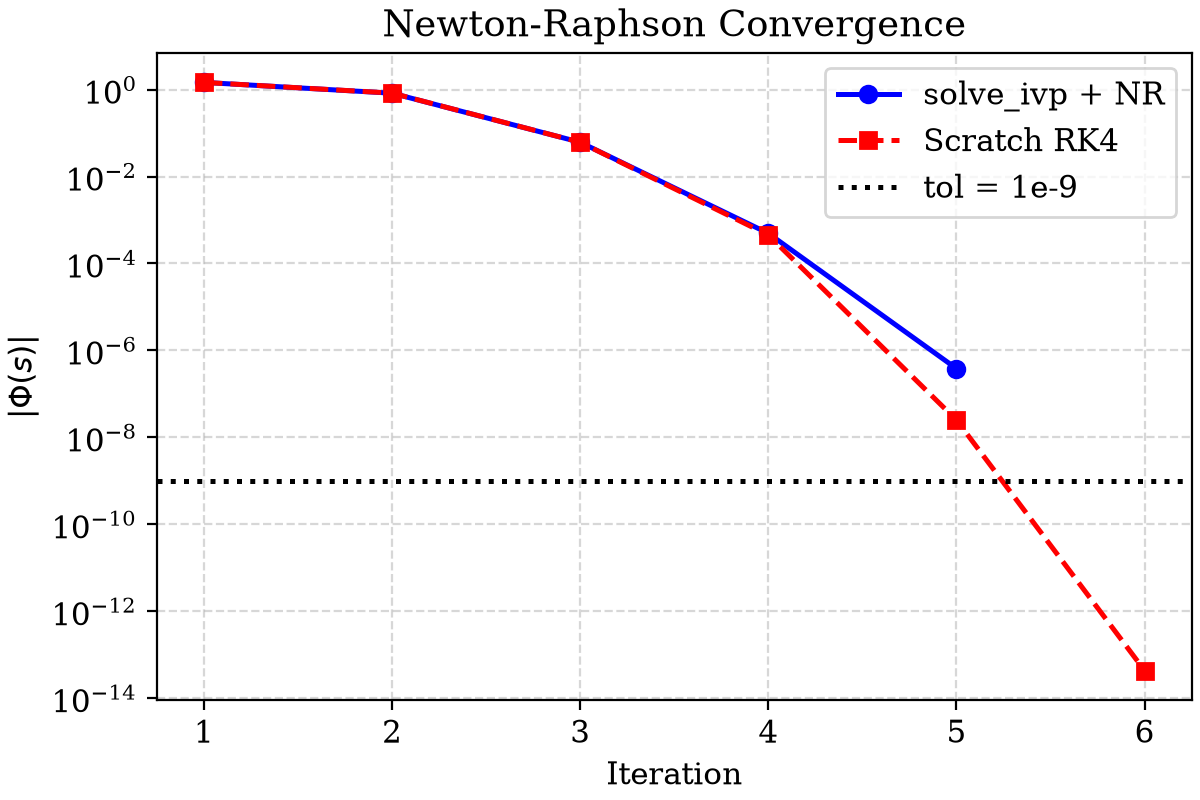
\includegraphics[width=\textwidth]{figures/newton_convergence.png}
        \caption{Convergence of Newton--Raphson iterations.}
        \label{fig:newton}
    \end{subfigure}
    \hfill
    \begin{subfigure}[b]{0.48\textwidth}
        \centering
        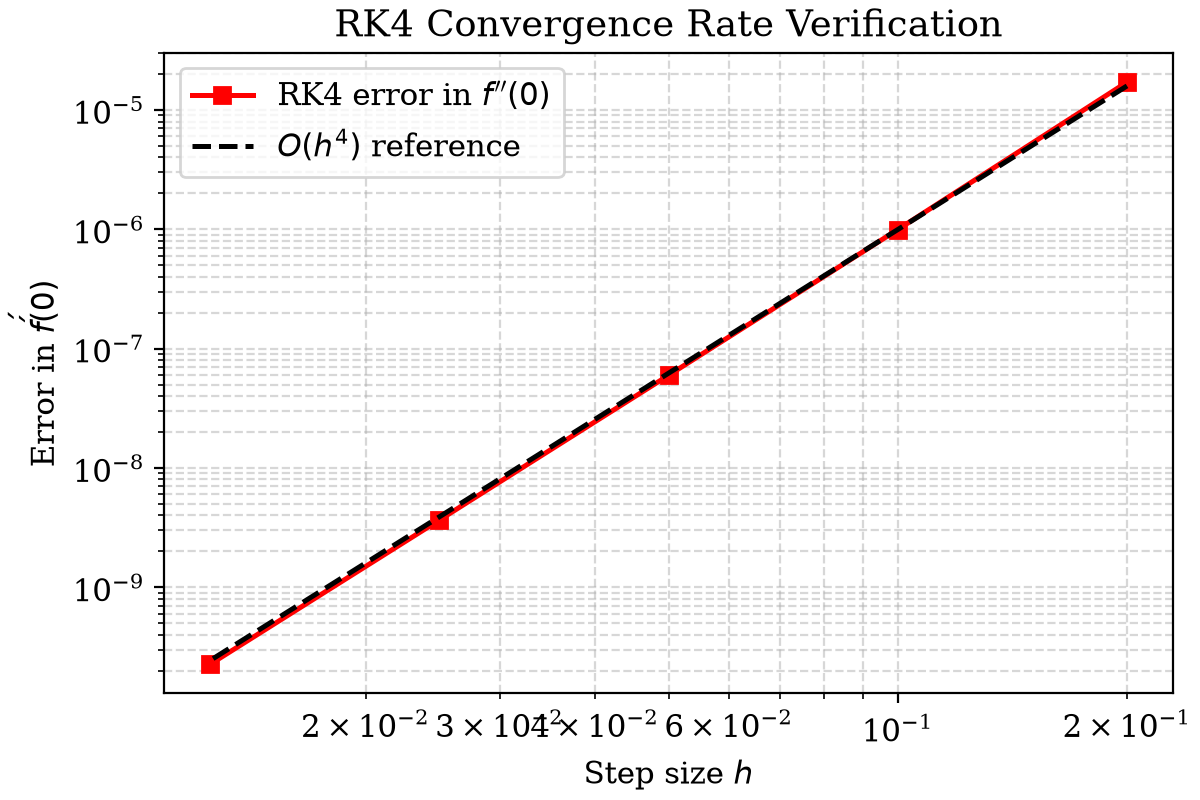
\includegraphics[width=\textwidth]{figures/rk4_convergence.png}
        \caption{RK4 error vs step size $h$, confirming $\mathcal{O}(h^4)$.}
        \label{fig:rk4}
    \end{subfigure}
    \caption{Convergence behavior of the shooting methods.}
\end{figure}

\subsection{Effect of Domain Truncation and RK4 Order of Accuracy}

Figure~\ref{fig:rk4} confirms that the scratch RK4 integrator achieves 4th-order accuracy: halving $h$ reduces the error by a factor of $\approx 16$. A domain truncation study (not shown) found that $\eta_\infty \geq 6$ is sufficient for the shooting methods; below $\eta_\infty \approx 5$, the artificial boundary distorts the solution.

% ----------------------------------------------------------------
\section{Conclusion}
% ----------------------------------------------------------------

Three distinct approaches were used to solve the Falkner--Skan stagnation point problem, all producing $f''(0) = 1.23258766$ to at least 10 decimal digits. The from-scratch RK4 approach is the most transparent, the \texttt{solve\_ivp} shooting method is the most accurate with exact sensitivity Jacobians, and \texttt{solve\_bvp} is the most robust to initial guesses. Integral quantities ($\delta^* = 0.6479$, $\theta = 0.2923$, $H = 2.216$) agree with textbook values.

\begin{thebibliography}{9}

\bibitem{hiemenz1911}
K.~Hiemenz, ``Die Grenzschicht an einem in den gleichförmigen Flüssigkeitsstrom eingetauchten geraden Kreiszylinder,'' \textit{Dinglers Polytech. J.}, 326:321--324, 1911.

\bibitem{falkner1931}
V.~M. Falkner and S.~W. Skan, ``Some approximate solutions of the boundary layer equations,'' \textit{Phil. Mag.}, 12(80):865--896, 1931.

\bibitem{schlichting2016}
H.~Schlichting and K.~Gersten, \textit{Boundary-Layer Theory}, 9th ed., Springer, 2016.

\bibitem{white2006}
F.~M. White, \textit{Viscous Fluid Flow}, 3rd ed., McGraw-Hill, 2006.

\end{thebibliography}

\end{document}
